%
% The first command in your LaTeX source must be the \documentclass command.
\documentclass[sigconf]{acmart}

%
% defining the \BibTeX command - from Oren Patashnik's original BibTeX documentation.
\def\BibTeX{{\rm B\kern-.05em{\sc i\kern-.025em b}\kern-.08emT\kern-.1667em\lower.7ex\hbox{E}\kern-.125emX}}
    
% Rights management information. 
% This information is sent to you when you complete the rights form.
% These commands have SAMPLE values in them; it is your responsibility as an author to replace
% the commands and values with those provided to you when you complete the rights form.
%
% These commands are for a PROCEEDINGS abstract or paper.
\copyrightyear{2018}
\acmYear{2018}
\setcopyright{acmlicensed}

\acmConference[SPLC'19]{23rd International Systems and Software Product Line Conference}{9--13 September, 2019}{Paris, France}
\acmBooktitle{Woodstock '18: ACM Symposium on Neural Gaze Detection, June 03--05, 2018, Woodstock, NY}
\acmPrice{15.00}
\acmDOI{10.1145/1122445.1122456}
\acmISBN{978-1-4503-9999-9/18/06}

%
% These commands are for a JOURNAL article.
%\setcopyright{acmcopyright}
%\acmJournal{TOG}
%\acmYear{2018}\acmVolume{37}\acmNumber{4}\acmArticle{111}\acmMonth{8}
%\acmDOI{10.1145/1122445.1122456}

%
% Submission ID. 
% Use this when submitting an article to a sponsored event. You'll receive a unique submission ID from the organizers
% of the event, and this ID should be used as the parameter to this command.
%\acmSubmissionID{123-A56-BU3}

%
% The majority of ACM publications use numbered citations and references. If you are preparing content for an event
% sponsored by ACM SIGGRAPH, you must use the "author year" style of citations and references. Uncommenting
% the next command will enable that style.
%\citestyle{acmauthoryear}

%
% end of the preamble, start of the body of the document source.
\begin{document}

%
% The "title" command has an optional parameter, allowing the author to define a "short title" to be used in page headers.
\title{Towards Automated Composition of a Product Line}

%
% The "author" command and its associated commands are used to define the authors and their affiliations.
% Of note is the shared affiliation of the first two authors, and the "authornote" and "authornotemark" commands
% used to denote shared contribution to the research.
\author{Shengmei Liu}
\email{sliu7@wpi.edu}
\affiliation{%
  \institution{WPI}
  \streetaddress{100 Institute Road}
  \city{Worcester}
  \state{Massachusetts}
  \postcode{01609}
}

\author{George T. Heineman}
\email{heineman@wpi.edu}
\affiliation{%
  \institution{WPI}
  \streetaddress{100 Institute Road}
  \city{Worcester}
  \state{Massachusetts}
  \postcode{01609}
}

%
% By default, the full list of authors will be used in the page headers. Often, this list is too long, and will overlap
% other information printed in the page headers. This command allows the author to define a more concise list
% of authors' names for this purpose.
% \renewcommand{\shortauthors}{Trovato and Tobin, et al.}

%
% The abstract is a short summary of the work to be presented in the article.
\begin{abstract}
Object-oriented (OO) frameworks represent a significant achievement in extensible design,
but there are many well-documented challenges when third-party programmers attempt to use and
refactor them. In earlier work, we described how to migrate existing OO framework- based software
into a software product line structure using combinatory logic synthesis (CLS) integrated into FeatureIDE,
an Eclipse-based IDE that supports feature-oriented software development. While initially successful at
synthesizing a few instances of a product line, the approach does not scale to support larger product
lines because it does not adequately capture the commonality and inherent variability in the application domain.
In this paper, we analyze these problems, and introduce our new approach to construct product line which
overcomes many drawbacks of old approach. We describe how application domain modeling helps automated
composition, and how our redesigned CLS-engine improves scalability. Results are illustrated by scaling
the well-known graph product line with our approach, while reducing the average amount of instance-specific
code significantly, generating more readable code and providing more convenience for refactoring.
\end{abstract}

%
% The code below is generated by the tool at http://dl.acm.org/ccs.cfm.
% Please copy and paste the code instead of the example below.
%

%
% Keywords. The author(s) should pick words that accurately describe the work being
% presented. Separate the keywords with commas.
\keywords{datasets, neural networks, gaze detection, text tagging}

%
% This command processes the author and affiliation and title information and builds
% the first part of the formatted document.
\maketitle

\section{Introduction}
%% 
%% Introduction
%%
%% Key ideas: 
%%
%% 1. Augmenting feature models with application domain modeling
%% 2. Impact this has on the toolsuite for featureIDE and composition engines
%%
%% 3. Expose programming API instead of providing a standard black-box
%%    capability, which might otherwise restrict users' abilities.

Software product lines (SPLs) refer to software engineering methods,
tools and techniques for creating a collection of similar software
systems, called product line members, from a shared set of software
assets using a common means of production. A number of characteristics
separate SPLs from routine large, complex systems and thus there is a need for specialized tools and techniques to design, implement and maintain SPLs. 

Fundamental to many SPL approaches is the concept of a \textit{Feature
Model}, first introduced by the Feature-Oriented Domain Analysis (FODA)
technique~\cite{Kang1990} and refined over the years by numerous
researchers. A feature model is composed of user-visible features from
which a wide variety of configurations can be defined through the
selection of individual features. Many tool chains have been developed
to generate product line members ``on demand'' from a feature model
configuration. Developers need to construct the SPL code artifacts in a
specific way that enables the tools to work; this may include, for
example, low-level compiler directives embedded in source code, or
specialized languages (such as JAK~\cite{Batory2004FeatureorientedPA} or
DeltaJ~\cite{Schaefer:2010:DPS:1885639.1885647}) that developers use to
encode the artifacts.

%%\begin{figure}
%%    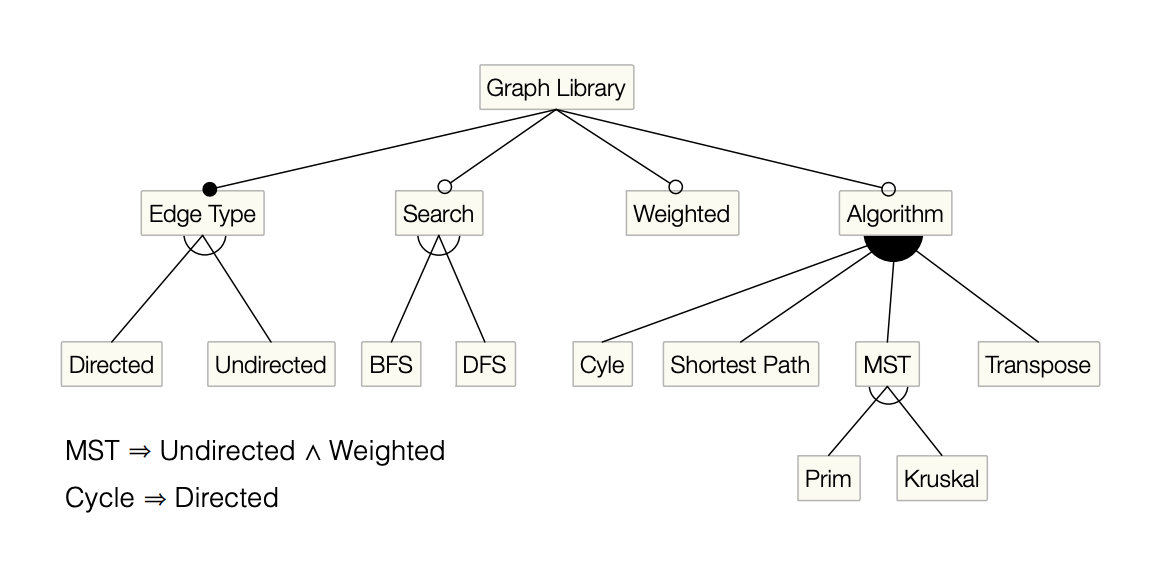
\includegraphics[scale=0.4,natwidth=1154,natheight=576]{gpl2.png}
%%    \caption{Graph Product Line Feature Model}
%%    \label{fig:feature-model}
%%\end{figure}

There remains a potential issue, however, when the variability inherent in the product line relates to the application domain model. The common result is that one must integrate these domain-model concepts into the feature model so they can become part of the configuration process. The feature model from Figure~\ref{fig:feature-model} contains features relating to behavior (i.e., \textbf{Prim} contains Prim's implementation of the Minimum Spanning Tree problem) and some relate to structure (i.e., \textbf{Weighted} captures the notion that edges in a graph may have weights). 

In past work, we have explored product lines within a number of application domains~\cite{Heineman:2015:TMO:2791060.2791076,PEPM18}

%We make the following observations regarding product lines:
%
%--
%
%--Should be able to add to and remove features from a product line after it has been defined
%
%--A product line definition is still reflected in software artifacts, which means it should support common refactoring functionality
%
%--Should be feature-rich, which means one can potentially envision a significant number of PL members (e.g., not just a handful)
%
%Without one of these characteristics, it could only be considered a closed system.


% A SPL is a family of related programs. When the units of program
% construction are feature—increments in program functionality or
%development—every program in an SPL is identified by a unique and legal
%combination of features, and vice versa. Family member refers to
%individual product. A variation point represents a decision leading to
%different variants of an asset. A variation point consists of a set of
%possible instantiations (legal variations of the variation point). A
%variation point usually specifies the binding times, that is the
%time/times at which a decision about the instantiation has to be taken.

%The variant derivation is the action in which assets are combined from
%the set of available assets and contained variation points are
%bound/instantiated. If there are variation points with multiple binding
%times, the derivation will happen stepwise at each binding time. The
%result of such a derivation is a set of derived assets. The derivation
%can be executed technically in many ways. The simplest way is to copy
%assets and modify (parts of) them (e.g. the configuration parameters)
%manually. The result of such a derivation is often called a
%configuration.



%% THESE NEED TO BE PLACED IN CONTEXT.
Here is a reference to K\"{a}stner's paper~\cite{Kastner:2012}.

Here is a reference to ~\cite{leich2005tool}.
Here is a reference to ~\cite{proksch2014tool}.
Here is a reference to ~\cite{7203038}.
Here is a reference to ~\cite{Sayre:2005:UMA:1082983.1083277}.
Here is a reference to ~\cite{Setyautami:2016:UPD:2934466.2934479}.
Here is a reference to ~\cite{Sousa:2016:EFM:2934466.2934475}.

Here is a reference to ~\cite{Arcaini:2017:ARV:3106195.3106206}.

Here is a reference to ~\cite{Vasilevskiy:2016:TRP:2934466.2934484}.

Here is a reference to ~\cite{Kuhn:2015:CPC:2791060.2791092}.

Here is a reference to ~\cite{Schaefer:2010:DPS:1885639.1885647}.

Here is a reference to ~\cite{Apel:2008:AFF:1428476.1428480}.


\subsection{Approaches to Product Line Development}

Software product lines create unique engineering challenges for a number
of reasons. First, it should be possible to generate any number of
instances of the product line, and by this we mean the code artifacts
for the instance application. These are then compiled (or interpreted)
to realize the execution of the application. Second, there are multiple
development efforts; one can work on code that will effectively be used
by all product line instances, but at other times, one is focused on
writing code for just a single instance from the PL.

A major goal of featured-oriented PL is to derive a product
automatically based on user’s selection. There are three philosophical
approaches widely used in practice -- \textit{annotation-based} ,
\textit{composition-based} or \textit{component-based} -- which differ
in the way they represent variability in the code base and the tool
chains used to generate the product line members.

\subsubsection{Annotation-based Approach}

An annotation-based SPLC consists of a single body of code artifacts
which fully contains all code resources used by all members of the
product line. Using different tools or language-specific capabilities, a
compiler (or pre-processor) extracts subsets of the code to be used for
a PL instance. One of the most common approaches is to use compiler
directives embedded within the code as a means for isolating code unique
to a subset of product line instances. Then each product line instance
can be generated by compiling the same code base with different compiler
flags, resulting in different executable instances. Due to the nature of
this approach, often one cannot review the source code for individual
instances.~\cite{Apel:2013:FSP:2541773}. Often the compiler directives
manipulate the core data structures or class definitions of the
software, for example, adding or removing a field definition~\cite{Liebig:2010:AVF:1806799.1806819}.

Annotation-based approaches are widely used in practice because they are
easy to use and already natively supported by many programming
environments. It keeps good readability and low complexity, however,
relatively simple tool support can address scattered code or
errors.~cite{Kastner:2012,Apel:2013:FSP:2541773}.


\subsubsection{Composition-based Approach}

Another approach is to design a feature tree which is used to capture all the externally visible features that
can be used to differentiated one product line instance from another. Then code assets are internally associated
 with each of these visible features. Finally product line instances are configured by selecting for inclusion
  features from the feature tree, potentially restricted by constraints. A composition engine processes the
  code assets associated with the selected features to create the final source code for the product line instance.

Composition-based approaches locate code belonging to a feature or feature combination in a dedicated file,
container, or module. A classic example is a framework that can be extended with plug-ins, ideally one plug-in
per feature. The key challenge of composition-based approaches is to keep the mapping between features and
composition units simple and tractable.

Another way to view the difference between annotation and composition is that annotation separate concerns
virtually and composition separate concerns physically,and code is removed on demand with annotation while
composition units are added on demand.

~\cite{Thum:2014:FEF:2537169.2537315,Apel:2013:FSP:2541773,Schaefer:2010:DPS:1885639.1885647
,Dhungana:2011:DMD:1924082.1924092,Heineman:2015:TMO:2791060.2791076,Batory2004FeatureorientedPA,
leich2005tool,Setyautami:2016:UPD:2934466.2934479,Ddder2013UsingII,Apel:2009:FLA:1555001.1555038,
proksch2014tool}.

\subsubsection{Component-based Approach}

A software component is a unit of composition with contractually specified interfaces and explicit context
dependencies only. A software component can be deployed independently and is subject to composition by third
parties. The key idea of a component is to form a modular, reusable unit.

Developing product line by constructing and composing reusable was a common strategy. With domain analysis,
developers decided which functionality should be reused across multiple products of the product line designed
components accordingly. To derive a product for a given feature selection during application engineering, a
developer selects suitable components and then manually writes glue code to connect components for every
product individually.

~cite{Kuhn:2015:CPC:2791060.2791092,atkinson2000component}.


\subsubsection{Product Line Techniques In Industry}

Annotation-based approach are not so widely used as composition-based approach because drawbacks mentioned above.
Here are some existing annotation-based approaches:

code coloring (FeatureCIDE): CIDE is an Eclipse plug-in that replaces the Java editor in SPL projects. Developers
start with a standard Java legacy application, then they select code fragment and associate them with features
 from the context menu. The marked code is then permanently highlighted in the editor using a background color
 associated with the feature. Here is a reference to ~\cite{CIDE:Eclipse}.


Type checking approach,  a product-line-aware type system that statically and efficiently detects type errors in
annotation-based product-line implementations.~\cite{Kastner:2012}


To work with FeatureIDE, the primary challenge is to design a feature tree model to represent the desired product
line application domain. Because features are cross-cutting with regards to the artifacts in the programming
language, the various composer engines supported by FeatureIDE accomplish the same goal in a variety of ways.

AHEAD has feature modules for each concrete feature, and the corresponding composition tool places generated
source code directly into the Eclipse source folder. AHEAD brings separate tools together and selects different
tools for different kinds of files during feature composition,establishing a clear interface to the build
system. Composing Jak files will invoke a Jak-composition, whereas composing XML files invokes an
XML-composition tool.~\cite{Batory2004FeatureorientedPA}.

FeatureHouse tool suite has been developed that allows programmers to enhance given languages rapidly with
support for feature-oriented programming. It is a framework for software composition supported by a
corresponding tool chain. It provides facilities for feature  composition based on a language-independent
model and tool chain for software artifact, and a plug-in mechanism for the integration of new artifact
languages.~\cite{Apel:2009:FLA:1555001.1555038}

Deltaj is a Java-like language which allows to organize classes in modules. A program consists of a base
 module and a set of delta module in a stepwise manner. Much like a feature module, a delta module can add
 new classes and members as well as extend existing methods by overriding. In contrast to feature modules,
 delta modules can also delete existing classes and individual members.~\cite{Schaefer:2010:DPS:1885639.1885647}.

In LaunchPad, each feature can contain any number of combinators, designed using a DSL we had developed to
simplify the writing of combinators for an earlier CLS tool. A configuration is a subset of features from
which a repository is constructed. Each feature can optionally store target definitions, which are aggregated
 together and then used as the basis for the inhabitation requests, i.e.As each request is satisfied, the
 synthesized code from the resulting type expression M is stored in the designated source folder.
~\cite{Heineman:2015:TMO:2791060.2791076}.

\subsubsection{Evaluation of related work}

The key challenge of composition-based approaches is to keep the mapping between features and composition units
simple and tractable. Preprocessor-based and parameter-based implementations are often criticized for their
potential complexity, lack of modularity, and reduced readability. And they all have some problems which is the
difficulty to refactoring.~\cite{Kim:2017:RJS:3106195.3106201}.

Although component-based implementations are common in product line practice, they lack the automation potential
of feature orientation that we aim at. Deciding when to build a reusable component and what to include in
that component is a difficult design decision, one need to have good understanding of whole scope to do that.
There is no domain in this approach, glue code is a necessary, it's no more than assembling components.
~\cite{Apel:2013:FSP:2541773}

In practice most PLs appear “from the ground up” where developers take advantage of language-specific capabilities
 to annotate different code regions as being enabled (or disabled) based on compiler directives. Starting from an
 annotation-based code repository many composition-based approaches simply “snipped” or refactored code fragments
 to recreate countless tiny “features” that could be selected.

Manual composition is a configuration process. A designer selects individual features from a feature model and
relies on constraints to ensure the resulting product line member is valid. Manual Composition is limited to a
potential total of 2N configurations where N represents the number of available features in the model. There is no
 domain modeling, What commonly occurs is the designer must make sure that changes to any of the units will not invalidate those product
 line members that incorporate that feature.

 Another problem is that the features are fixed and unchanging. If we need to make some modifications to current
 instances, we may need to trace all the way back and change the code in many classes because it’s inheritance
 structure. If we want to add features which is slightly different from existing ones, we may need to start from
 very beginning.


\section{A New Approach is Needed}
% New Approach % As we investigated the way in which application domains
were represented in feature models, we identified a number of
limitations in how modeling was represented and devised a number of
strategies for improving the way these application domain models could
improve the process of generating product line members.

There are features to represent the structure of a variations, and there
is a feature for each variation. Our goal was to support the easy
construction of new variations by reusing existing features where
possible and adding new features as needed to support the functionality
expected of new variations.

\subsection{Integrated application domain models}

The concept of an application domain model is common in software
engineering because of its ability to identify real-world concepts that
will ultimately be present in a software system. When the model is
actively maintained over time, as changes are introduced and the
software system evolves, there is the opportunity to take advantage of
its high-quality information.

Annotation-based approaches for SPLs that rely solely on the embedded
compiler directives within the code are incompatible with a separately
designed application domain model. When product lines use compiler
directives to alter the very structure of the object-oriented classes in
the code base, as observed in~\cite{Kastner:2012}, there needs to be
extensive type checking to ensure only valid product line members are
generated. In these cases, one typically finds that ``the code is the
design'' and there no other separate representation of the classes being
manipulated by the compiler directives. For this reason, our
investigation focused primarily on composition-based SPLC approaches.

The application domain modeling is still problematic on both feature model
system and Object-oriented system. The feature model system is no more than
a closed feature tree system, with features encapsulated in black boxes. It's a
full model that we plan every detail of the model in advance, with no guarantee that the
code generated eventually will work. It's hard to deal with domain variability and extension.
We can only add features into the system who doesn't change the structure.
In the Object-oriented system, the configuration becomes
 hard that there are no boxes of features for us to choose from. Though
we can utilize UML or MDE for modeling, it relies on deep understanding and proficient using of various
tools. The limitation of tools would finally restrict it's ability.
Type safe problem is also a widely discussed problem with modeling of OO system.

Researchers have investigated various object-oriented technologies to
support SPLs~\cite{Griss1999,Batory2000} with the focus of finding ways
to develop reusable components within an SPLC, whether using variations
of \textit{mixins}~\cite{Bracha:1990:MI:97946.97982} or C++
Templates~\cite{VanHilst:1996:UCT:646898.710025}. What is missing,
however, is the capability for the application domain model to be fully
integrated into the SPLC tool chain and have as great an influence as
the features themselves. We observed in nearly every approach using
feature models that the lack of a domain model resulted in increasingly
complicated feature models.This is most
evident when reviewing sample product lines as supported by
FeatureIDE~\ref{Thum:2014:FEF:2537169.2537315}, an extensible
Eclipse-based framework for feature-oriented software development. A
product line member is defined solely by the configuration of existing
features in the feature model, as allowed by the defined constraints.
Because there is no separate domain model, the various FeatureIDE
approaches all appear to have configurations which become ineffective
domain modeling. For example, in some FeatureIDE models, there are
features with sub-features that appear to be nothing more than
instantiations of different configurations,as we first identified in Figure~\ref{fig:feature-model}.  which does little to reduce
the overall complexity, and instead, simply widens the feature model tree.

In our approach, we realized lightweight partial modeling and code synthesis.
We don't have to model the full domain in the first place like feature model system,
or rely on tool sets that much like OO system. We simply model the part we want and synthesize
code.

\subsection{CLS generic composition}

With dominated approach for using feature in PLs, n features in the
feature tree may generate 2n configurations which will become product
line instances. But if we use CLS as the algorithm for composition, the
fundamental units will be combinators instead of features. The CLS
starts with a repository of combinators to which a user issues a query
which attempts to find a type in the repository using inferencing. Using
CLS generic composition, limitations of composition tools are
eliminated.


Combinators can be dynamic and added at composition time, something
which is simply not possible in traditional feature trees used by
feature-oriented product lines.

To better explain these dynamic combinators, consider having a feature
model with a feature that provides variability and there are a number of
fixed sub-features that are tailored for each valid variation. For
example, “Number of external hard disks” might have sub-features
“One-Hard-Disk”, “Two-hard-disks” and so on. Individual members of the
PL are configured, accordingly, to select the desired number of external
hard disks. In contrast, using CLS a single combinator class
NumberOfExternalDisks is parameterized with an integer, and one can
instantiate a combinator (NumberOfExternalDisks(3)) and add to the
repository as needed based on the modeling needs of the member.

Without making 2n configurations, using CLS will significantly simplify
code system in PL, optimize code structure make it more readable and
reasonable.


\subsubsection{Compositional manipulation}

Feature-IDE relies on externally provided composition engines to process
code fragments. The challenge is that FeatureIDE can make no semantic
guarantees about the resulting code. Also there is no theoretical
foundation for the composition, which rather simply is assembly. During
assembly, units are wired together without making any changes to the
units themselves.

\subsubsection{Language agnostic}


Without being language limited as normal ways, our approach is more
laguage agnostic. Choice of language have been more diversified, which
could benefit more engineers with different backgrounds. We don't have
to take advantage of single language to build our code base. For
example,we have to use .jak files in AHEAD. If you are not familiar with
the language, you can't use the approach.~\cite{PEPM18}.

\subsubsection{Code sharing between assets}


Like we mentioned above, dynamic combinators can be constructed to add
methods into classes. Assets can share some basic code, with different
methods included.


\section{Graph Product Line}
%% Here is where to describe GPL


The Graph Product Line (GPL) is a well-known case study within the software product line community. This product line
 supports variations in a library of graph data strutures and algorithms. A possible feature diagram of the graph
 library is shown in Figure?. The root is labeled with Gpl to represent a graph product. It has a mandatory child feature
 GraphType, because each graph library has to implement an type, which is either Directed or Undirected. Furthermore,
 three other child features of the root are optional: Search, Weighted and Algorithm. Search strategies may be either
  breadth-first search (BFS) or depth-first search (DFS). Algorithm offers a selection of graph algorithms as child
  features. Since it's optional, either zero, one, ore more algorithms may be presented in a graph product. In our
  example, the algorithm for minimal spanning trees MST has two alternative implementations, Prim and Kruskal. Some
  non-local conditions are modeled as explicit Boolean constraints-- for example, minimal spanning tree make only
  sense for weighted graphs, and shortest paths can be computed directed graphs only.


\section{Design of CLS-based GPL}
The design of the CLS-based GPL goes here...

\section{Evaluation}
Evalution of our approach goes here...

\section{Conclusion}
We conclude in this section...

Also talk about future work



\section{Acknowledgments}

Identification of funding sources and other support, and thanks to individuals and groups that assisted in the research and the preparation of the work should be included in an acknowledgment section, which is placed just before the reference section in your document. 

This section has a special environment:
\begin{verbatim}
  \begin{acks}
  ...
  \end{acks}
\end{verbatim}
so that the information contained therein can be more easily collected during the article metadata extraction phase, and to ensure consistency in the spelling of the section heading. 

Authors should not prepare this section as a numbered or unnumbered {\verb|\section|}; please use the ``{\verb|acks|}'' environment.

\section{Appendices}

If your work needs an appendix, add it before the ``\verb|\end{document}|'' command at the conclusion of your source document. 

Start the appendix with the ``\verb|appendix|'' command:
\begin{verbatim}
  \appendix
\end{verbatim}
and note that in the appendix, sections are lettered, not numbered. This document has two appendices, demonstrating the section and subsection identification method.

\section{SIGCHI Extended Abstracts}

The ``\verb|sigchi-a|'' template style (available only in \LaTeX\ and not in Word) produces a landscape-orientation formatted article, with a wide left margin. Three environments are available for use with the ``\verb|sigchi-a|'' template style, and produce formatted output in the margin:
\begin{itemize}
\item {\verb|sidebar|}:  Place formatted text in the margin.
\item {\verb|marginfigure|}: Place a figure in the margin.
\item {\verb|margintable|}: Place a table in the margin.
\end{itemize}

%
% The acknowledgments section is defined using the "acks" environment (and NOT an unnumbered section). This ensures
% the proper identification of the section in the article metadata, and the consistent spelling of the heading.
\begin{acks}
To Robert, for the bagels and explaining CMYK and color spaces.
\end{acks}

%
% The next two lines define the bibliography style to be used, and the bibliography file.
\bibliographystyle{ACM-Reference-Format}
\bibliography{splc19}

% 
% If your work has an appendix, this is the place to put it.
\appendix

\section{Research Methods}

\subsection{Part One}

Lorem ipsum dolor sit amet, consectetur adipiscing elit. Morbi malesuada, quam in pulvinar varius, metus nunc fermentum urna, id sollicitudin purus odio sit amet enim. Aliquam ullamcorper eu ipsum vel mollis. Curabitur quis dictum nisl. Phasellus vel semper risus, et lacinia dolor. Integer ultricies commodo sem nec semper. 

\subsection{Part Two}

Etiam commodo feugiat nisl pulvinar pellentesque. Etiam auctor sodales ligula, non varius nibh pulvinar semper. Suspendisse nec lectus non ipsum convallis congue hendrerit vitae sapien. Donec at laoreet eros. Vivamus non purus placerat, scelerisque diam eu, cursus ante. Etiam aliquam tortor auctor efficitur mattis. 

\section{Online Resources}

Nam id fermentum dui. Suspendisse sagittis tortor a nulla mollis, in pulvinar ex pretium. Sed interdum orci quis metus euismod, et sagittis enim maximus. Vestibulum gravida massa ut felis suscipit congue. Quisque mattis elit a risus ultrices commodo venenatis eget dui. Etiam sagittis eleifend elementum. 

Nam interdum magna at lectus dignissim, ac dignissim lorem rhoncus. Maecenas eu arcu ac neque placerat aliquam. Nunc pulvinar massa et mattis lacinia.

\end{document}
